\documentclass[tikz,border=5pt]{standalone}
\usepackage{tikz}
\usepackage{amsmath}
\usetikzlibrary{arrows.meta}
\definecolor{nebula}{HTML}{6366F1}
\definecolor{spark}{HTML}{14B8A6}
\definecolor{ink}{HTML}{334155}
\begin{document}
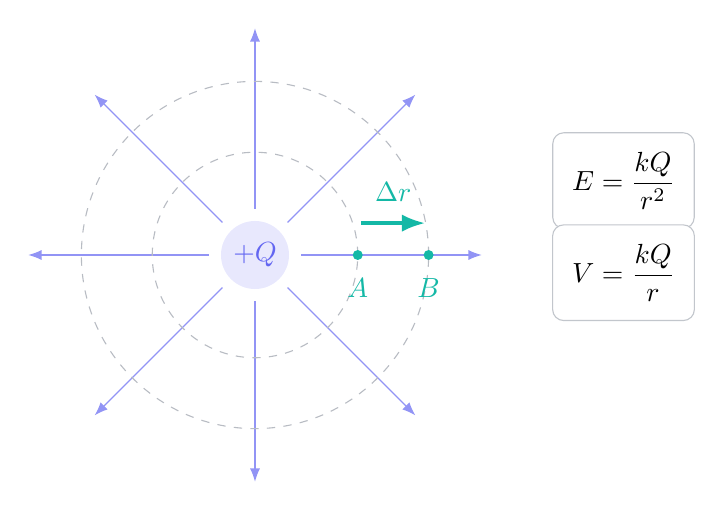
\begin{tikzpicture}[font=\sffamily,>=Latex,scale=.9]
  \fill[nebula!15] (0,0) circle (.48);
  \node[text=nebula,font=\bfseries] at (0,0) {$+Q$};
  \foreach \a in {0,45,...,315}{\draw[->,nebula!70] (\a:.65)--(\a:3.2);}
  \draw[dashed,ink!35] (0,0) circle (1.45);
  \draw[dashed,ink!35] (0,0) circle (2.45);
  \fill[spark] (1.45,0) circle (2pt) node[below=5pt] {$A$};
  \fill[spark] (2.45,0) circle (2pt) node[below=5pt] {$B$};
  \draw[->,very thick,spark] (1.5,.45)--(2.4,.45) node[midway,above=4pt] {$\Delta r$};
  \node[draw=ink!30,rounded corners=4pt,fill=white,inner sep=7pt] at (5.2,1.05)
    {$E=\dfrac{kQ}{r^2}$};
  \node[draw=ink!30,rounded corners=4pt,fill=white,inner sep=7pt] at (5.2,-.25)
    {$V=\dfrac{kQ}{r}$};
\end{tikzpicture}
\end{document}
